\documentclass{article}
\usepackage{float}
\usepackage{soul}
\usepackage{color} % Optional: to change highlight color
\usepackage{subcaption}
\captionsetup{font=small,labelfont=bf}
\sethlcolor{yellow} % Sets highlight color



% if you need to pass options to natbib, use, e.g.:
%     \PassOptionsToPackage{numbers, compress}{natbib}
% before loading neurips_2026

% The authors should use one of these tracks.
% Before accepting by the NeurIPS conference, select one of the options below.
% 0. "default" for submission
% \usepackage{neurips_2026}
% the "default" option is equal to the "main" option, which is used for the Main Track with double-blind reviewing.
% 1. "main" option is used for the Main Track
%  \usepackage[main]{neurips_2026}
% 2. "position" option is used for the Position Paper Track
%  \usepackage[position]{neurips_2026}
% 3. "eandd" option is used for the Evaluations & Datasets Track
 % \usepackage[eandd]{neurips_2026}
 % if you want to opt-in for a de-anomymized submission (not recommended, but OK):
 % \usepackage[eandd, nonanonymous]{neurips_2026}
% 4. "creativeai" option is used for the Creative AI Track
%  \usepackage[creativeai]{neurips_2026}
% 5. "sglblindworkshop" option is used for the Workshop with single-blind reviewing
 % \usepackage[sglblindworkshop]{neurips_2026}
% 6. "dblblindworkshop" option is used for the Workshop with double-blind reviewing
%  \usepackage[dblblindworkshop]{neurips_2026}

% After being accepted, the authors should add "final" behind the track to compile a camera-ready version.
% 1. Main Track
 % \usepackage[main, final]{neurips_2026}
% 2. Position Paper Track
%  \usepackage[position, final]{neurips_2026}
% 3. Evaluations & Datasets Track
 % \usepackage[eandd, final]{neurips_2026}
% 4. Creative AI Track
%  \usepackage[creativeai, final]{neurips_2026}
% 5. Workshop with single-blind reviewing
%  \usepackage[sglblindworkshop, final]{neurips_2026}
% 6. Workshop with double-blind reviewing
%  \usepackage[dblblindworkshop, final]{neurips_2026}
% Note. For the workshop paper template, both \title{} and \workshoptitle{} are required, with the former indicating the paper title shown in the title and the latter indicating the workshop title displayed in the footnote.
% For workshops (5., 6.), the authors should add the name of the workshop, "\workshoptitle" command is used to set the workshop title.
% \workshoptitle{WORKSHOP TITLE}

% "preprint" option is used for arXiv or other preprint submissions
 \usepackage[preprint]{neurips_2026}

% NeurIPS sty uses \AtBeginDocument{\newgeometry{...}} so plain
% \geometry calls in the preamble get overridden. We override AFTER
% \maketitle below instead.

% to avoid loading the natbib package, add option nonatbib:
%    \usepackage[nonatbib]{neurips_2026}

\usepackage[utf8]{inputenc} % allow utf-8 input
\usepackage[T1]{fontenc}    % use 8-bit T1 fonts
\usepackage{hyperref}       % hyperlinks
\usepackage{url}            % simple URL typesetting
\usepackage{booktabs}       % professional-quality tables
\usepackage{amsfonts}       % blackboard math symbols
\usepackage{amsmath}
\usepackage{amssymb}
\usepackage{nicefrac}       % compact symbols for 1/2, etc.
\usepackage{microtype}      % microtypography
\usepackage{xcolor}         % colors
\usepackage{graphicx}
\usepackage{wrapfig}
\usepackage{cleveref}
\usepackage{titlesec}
% tighter section / subsection / paragraph spacing so the document
% packs more text per page and section breaks don't waste vertical space
\titlespacing*{\section}{0pt}{1.2ex plus 0.3ex minus 0.2ex}{0.6ex plus 0.2ex}
\titlespacing*{\subsection}{0pt}{0.9ex plus 0.2ex minus 0.1ex}{0.4ex plus 0.1ex}
\titlespacing*{\paragraph}{0pt}{0.5ex plus 0.1ex}{0.4em}

% tighter float spacing so figures and tables don't leave big gaps
% above and below themselves. Defaults are ~12-20pt; we drop those to
% near zero so figures sit close to surrounding text.
\setlength{\textfloatsep}{2pt plus 1pt minus 1pt}
\setlength{\intextsep}{2pt plus 1pt minus 1pt}
\setlength{\floatsep}{2pt plus 1pt minus 1pt}
\setlength{\abovecaptionskip}{2pt}
\setlength{\belowcaptionskip}{1pt}
% allow more aggressive vertical filling so LaTeX doesn't pad pages
% with whitespace when content nearly fills them
\renewcommand{\topfraction}{0.95}
\renewcommand{\bottomfraction}{0.95}
\renewcommand{\textfraction}{0.05}
\renewcommand{\floatpagefraction}{0.85}
% prevent LaTeX from stretching paragraph gaps vertically to fill pages.
% leftover space drops to the page bottom instead.
\raggedbottom

% Note. For the workshop paper template, both \title{} and \workshoptitle{} are required, with the former indicating the paper title shown in the title and the latter indicating the workshop title displayed in the footnote. 
\title{Predicting the Next Best Track in a DJ Set}


\author{%
  \textbf{Lavinia Elser}$^{1}$ \quad \textbf{Saurish Kapoor}$^{1}$ \quad  \\ \textbf{Johnathan Rafailov}$^{1}$ \quad \textbf{Jasmine Hanjra}$^{1}$ \\
  $^{1}$ Courant Institute of Mathematical Sciences \\
  New York University\\
  \texttt{\{le2396,sk12995,rafaij01,jh10489\}@nyu.edu} \\
}

\begin{document}
% Override NeurIPS default geometry. Wider text column (6.5in vs 5.5in
% default) packs more characters per line so paragraphs use fewer lines
% vertically. \newgeometry must run BEFORE \maketitle, otherwise it
% issues an implicit \clearpage that pushes the abstract to page 2.
\newgeometry{textwidth=6.5in, textheight=9.4in, top=0.85in,
             headheight=12pt, headsep=15pt, footskip=25pt}

\maketitle

\begin{abstract}
DJs spend countless hours combing through their music libraries to find songs that mix well together, taking time away from the craft of executing seamless transitions. We address this problem by training a recommendation system that takes a song's audio features as input and ranks the entire corpus by mixability, surfacing the most compatible candidates for mixing to the top. Unlike existing music recommenders that rely on user taste, genre, or artist metadata, we trained our models exclusively on \emph{acoustic properties}. We framed the task as binary pair classification, with positive pairs drawn from real DJ transitions and negative pairs sampled from non-transitions. We compared six models including Random Forest, Gradient Boosting, LightGBM, PCA with Random Forest, and a Siamese contrastive network. LightGBM achieved the highest test accuracy at $78.6\%$ under random negative sampling, with harmonic BPM distance and tempo emerging as the most predictive features. A survey of 35 participants ($20\%$ professional DJs) reported $67.84\%$ overall satisfaction with the recommended tracks.
\end{abstract}


\section{Introduction}

Disc jockeying can be an intense job. During a set, a DJ is required to read the room, manage its energy, work the crowd, and find the next song that will mix cleanly from the one currently playing. This all occurs within the runtime of a track, usually not lasting more than four minutes. Indeed, the choice of the next song is consistently consequential, and yet also the most repetitive. Most DJs work from personal libraries of thousands of tracks, often poorly annotated, and a meaningful amount of time from every set, or in preparation, is spent curating their playlists rather than planning the mixing. The motivation for building our model herein is to allow the DJ to spend more time of their set on mixing rather than retrieving. 

The model created acts a recommendation platform for DJs to facilitate the choice of the next track to play based on audio features derived from the track itself. Given a library of $N$ tracks and a query song $s$ the DJ is actively playing, the model ranks the remaining $N - 1$ tracks by how mixable each one is with the query $s$, and returns the corpus of library $N - 1$ ranked by mixability. 

We frame this as a supervised learning problem, where we believe a transition is executed well when the two tracks have similar tempos, comparable energy, and compatible rhythmic structures. Some common reasons a transition can be perceived as bad are large BPM jumps, incoherent loudness and intensity shifts, and clashing rhythmic structures (drums and onset layers poorly aligned during fadein and fadeout.)

Our paradigm thus attempts to solve a problem much different than traditional music recommendation platforms. Spotify-style recommendations rely on genre, playlist aggregation, and user-listening behavior, which are music metadata and potentially useful for discovery or maximizing end-user listening time, but do not invoke notions of mixability or transition quality. That said, we are solving a very different problem. To get a "mixability" signal, we train a pair classifier on a musical corpus, which contains adjacent transitions from thousands of real DJ sets. Positive pairs are real DJ transition pairs while negative pair sampling depends on two strategies in our approach. We split at the mix level rather than the track level to ensure no mix contributes to both train and test sets. Finally, we evaluate several model families for performance and report retrieval metrics relative to ground truth, as well as human evaluation metrics. Results from the survey show overall $67.84 \%$ satisfaction for the recommended tracks.


\section{Related Work}
Music recommendation systems combined with automatic mixing are projects that have been carried out previously, however, these investigated a slightly different problem than ours.

Systems like the one studied in \citep{aljanaki2017benchmark} are built around emotional tags and listener behavior, they are trying to predict what a person might enjoy based on their profile history, which makes sense for a streaming platform, but a DJ needs more than that. This system takes audio features as input and uses recurrent neural networks to predict the emotional dimensions of a song, specifically valence and arousal. This is quite different from what we are doing, where we focused on the mixability of two songs using their audio features, Which means that the tempo, energy, rhythm and overall song should fit well enough for the transition to feel natural. 

Work has also been done in creating automatic DJ systems \citep{arxiv2021autodj} that deal with transitions and beat matching, which is closer to what we are doing. The system uses a Generative Adversarial Network (GAN) in which the generator learns to mix tracks by applying equalization and fader features, while the discriminator evaluates if the generated transition resembles one from a real DJ mix. Cue points are automatically selected using an estimation of key and tempo. However, the outcome of this project is simply the mixes themselves, which contrasts to what we are trying to do which is to preserve model interpretability by exposing feature importances. This enables a DJ to be the final decision maker on what songs to select within the mix, allowing for personal judgment and individual taste to affect the final song selection.

Deej-AI \citep{teticio_deejai} is the most similar project to ours. It uses audio features instead of just looking at metadata. It uses a CNN trained on Mel spectrograms of 30-second audio clips to learn acoustic embeddings and combines this with a Track2Vec embedding trained on Spotify playlist co-occurrence to balance acoustic similarity with artist familiarity. However, this project trained on Spotify playlists, and so its objective is different from our project as it considers information about playlists, including song popularity and count across playlists in addition to song properties. However, DJs still need to know more about the properties of the song itself, as two songs can sound similar and still be a bad mix if the BPMs do not line up or the energy shift feels off.

\section{Methods}

\subsection{Dataset}

We use the open \emph{mir-aidj djmix-dataset} \citep{mir_aidj_djmix} as our source of real DJ transitions. The data set aggregates 5{,}040 MixesDB DJ mixes that are annotated by the community and includes 63{,}038 unique tracks and 64{,}753 adjacent track transitions. Each mix entry has an ordered tracklist with track titles, positions in the mix, and a YouTube source URL for the mix audio. Since the dataset only contains the metadata about the songs itself, we needed to scrape the audio files for the individual tracks separately.

Audio acquisition: We first filtered the tracks by songs that appear in at least three distinct mixes so that the model could learn contextual patterns about the songs rather than choosing songs that only exist in a single mix, which contains no contextual patterns about how the song was mixed. This collapses the long tail of the song distribution by mix and reduces the number of songs to approximately 4{,}100 tracks. We then queried YouTube (non-commercial academic analysis) for the corresponding song in our list and downloaded the audio with \texttt{yt-dlp} \citep{ytdlp}. Around 10--20\% of songs couldn't be downloaded for various reasons (404 error, age restrictions, etc.). After this stage, we had 3{,}827 tracks with usable audio.

Cleaning the tracklist metadata: A fraction of rows in our dataset had song titles that could not be parsed cleanly into an artist::title pair (formatting was inconsistent across mixes), and some unique track strings were near-duplicates of others (whitespace, ``feat.'' versus ``ft.'', artist order). We collapsed near-duplicate titles into one row, and we deleted any tracks we couldn't look up in our audio features table. If a track C in a mix [A, B, C, D] was unparseable or missing audio features, we kept (A,B) and dropped (B,C) and (C,D), rather than bridging across C by treating (B,D) as adjacent. A positive is therefore defined as a \textit{real observed transition}. We also dropped pairs in which the same track appeared on both sides, since these reflect annotation errors.

Considerations during selection: Two principles guided the choices above. First, we preferred the djmix-dataset over scraping 1001Tracklists or building our own corpus because its metadata is openly redistributable and tracklist information is kept separate from audio acquisition. Second, every cleaning step only removes rows. We drop tracks rather than fill in features, drop pairs rather than bridge missing tracks, and drop unmatched titles rather than guess at matches. The resulting set of positives is smaller, but each one is a transition a human DJ actually played, between songs that appear numerous times across the corpus.

\begin{figure}[h]
  \centering
  \begin{minipage}[c]{0.70\linewidth}
    \centering
    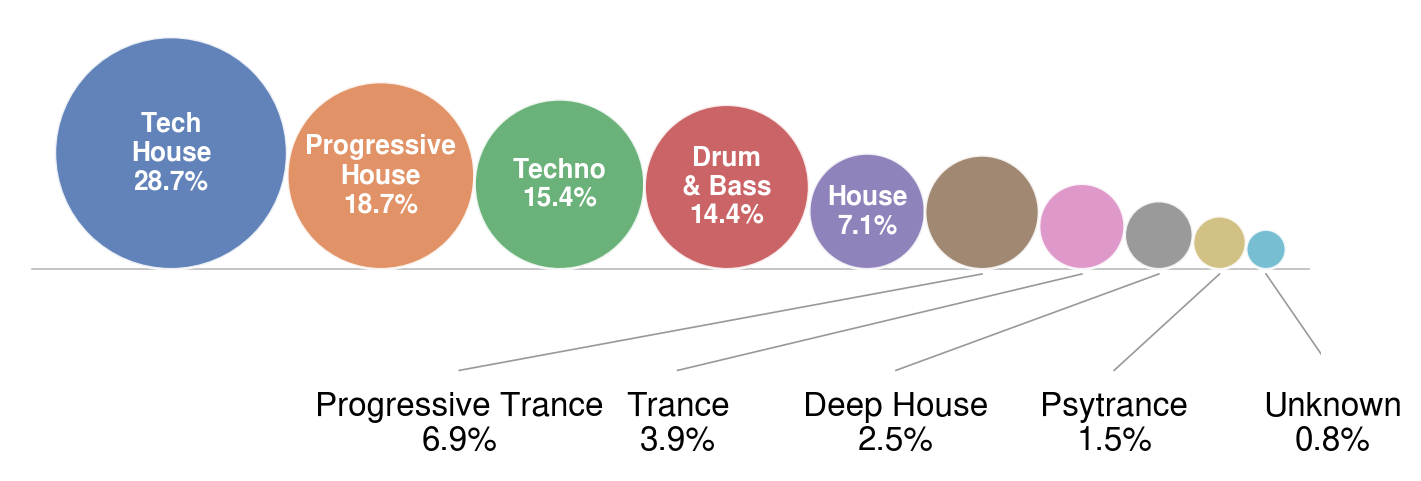
\includegraphics[width=\linewidth]{figures/genre_distribution_stacked.png}
  \end{minipage}%
  \hfill
  \begin{minipage}[c]{0.28\linewidth}
    \caption{Genre mix of the 3{,}827 tracks in the audio features table, derived from MixesDB tags propagated through the mixes each track appears in. Each circle is one of the top-10 genres; circle area is proportional to track count.}
    \label{fig:corpus-genres}
  \end{minipage}
\end{figure}

Final dataset. Of the 64{,}753 raw transitions, 3{,}724 had both endpoint tracks present in the audio features table; after dropping self-loops we retained 3{,}721 positive pairs spanning 1{,}605 distinct mixes. We sample negative pairs at a 1:1 ratio, giving a total of 7{,}442 labelled pairs. We split at the mix level, holding out 20\% of contributing mixes for testing so that no mix appeared in both partitions. The resulting partition contained 5{,}940 training pairs and 1{,}502 test pairs. The corpus skews heavily toward Tech House and Progressive House (\Cref{fig:corpus-genres}), which becomes a relevant detail when interpreting per-genre survey scores later on.



\subsection{Feature Extraction}

We extracted acoustic features from every .mp3 file with the librosa Python package \citep{mcfee2015librosa}, summarizing each per-frame time series into per-track means and standard deviations. The raw extraction produced a 1{,}602-column feature table; we then restricted the modeling input to ten feature families so that highly correlated raw representations such as \texttt{melspectrogram} and \texttt{chroma\_stft} did not dominate. The kept families cover three musical dimensions central to DJ practice: tempo (\texttt{tempo}, \texttt{tempogram\_ratio}), energy and rhythmic texture (\texttt{rms}, \texttt{zero\_crossing\_rate}), and spectral / harmonic / timbral content (\texttt{spectral\_centroid}, \texttt{spectral\_bandwidth}, \texttt{spectral\_contrast}, \texttt{spectral\_flatness}, \texttt{chroma\_cens}, \texttt{tonnetz}, \texttt{mfcc}). After filtering, each track is represented by a 113-dimensional feature vector.

DJs mix at three rhythmically compatible speeds: same tempo (1:1), double-tempo (2:1), and half-tempo (1:2). To capture this directly, we engineered a custom feature called \emph{harmonic BPM distance}, defined as:

\begin{equation}
\label{harmonicBPM}
    H_{BPM} = \min(|T_A - T_B|, |T_A - 2T_B|, |T_A - T_B/2|)
\end{equation}

Given a song $A$ with tempo $T_A$ and a song $B$ with tempo $T_B$, minimizing each term of \cref{harmonicBPM} leads to a perfect superposition of the two tracks under any of the three ratios.

\subsection{Pair Construction and Negative Sampling}

To finalize the construction of our dataset and make it ready for training, the next step was to determine the target variable. Since we wanted to recommend songs with high predicted mixability, we framed this recommendation task as a binary pair classification problem. We represent each pair as a feature vector $[A, B, |A - B|, H_{BPM}(A, B)]$, where $A$ and $B$ are the per-track librosa features. The absolute difference $|A-B|$ encodes how the two tracks differ across each feature, while $H_{BPM}$ captures harmonic tempo compatibility between the two songs.

Positive pairs are drawn from observed adjacent transitions in the DJ Mix Dataset: if two songs were played one after the other in the same mix, they are considered a positive pair.

Negative pairs require a sampling strategy, since not all non-transitions are equally informative about whether two songs are incompatible. We evaluated two strategies:

\begin{enumerate}
\item \textbf{Random negatives}: Two tracks sampled uniformly at random from the track pool, with the constraint that the pair is not a known positive transition in either direction.
\item \textbf{Hard negatives}: For each positive anchor track, we sample a candidate within $\pm 5$ BPM that is not a known transition. This forces the model to learn distinctions beyond simple BPM matching.
\end{enumerate}

To assess the compatibility of each negative sampling strategy with our engineered harmonic BPM distance feature, we computed the mean and median harmonic distance across positive and negative pairs under each strategy. The results are shown in \Cref{fig:hbpm-comparison}.

\begin{figure}[h]
    \centering
    \begin{minipage}[c]{0.32\linewidth}
        \centering
        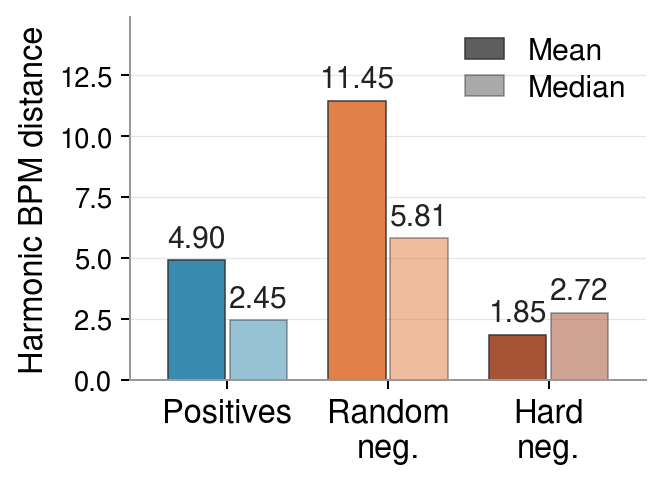
\includegraphics[width=\linewidth]{figures/harmonic_bpm_comparison.png}
    \end{minipage}%
    \hfill
    \begin{minipage}[c]{0.65\linewidth}
        \caption{Harmonic BPM distance for positives and negatives under each sampling regime. Random negatives sit well above positives, so the feature is a strong discriminator. Hard negatives, constrained within $\pm 5$ BPM of a positive anchor, invert the relationship by construction and eliminate the cue.}
        \label{fig:hbpm-comparison}
    \end{minipage}
\end{figure}

Under random negative sampling, the harmonic BPM distance feature carries strong discriminative signal: positive pairs have substantially lower harmonic distance than negatives. Under hard negative sampling, this relationship inverts, with negatives showing a smaller mean harmonic distance than positives. This is a direct consequence of the hard sampling constraint, which by construction selects negatives that are BPM-similar to a positive anchor. Because harmonic BPM distance is a feature we engineered specifically to capture the tempo compatibility that DJs rely on when choosing tracks, we chose random negative sampling for our primary pipeline. Hard negatives remain valuable as a stricter evaluation strategy that removes the easy BPM cue, and we report results under both strategies in Section 4 to provide a complete picture of model performance.

\subsection{Models}

We trained six models on the binary pair classification task.

\noindent\textbf{(1) Random Forest, default.} 100 trees, no maximum depth, default sklearn settings. This serves as our baseline. We chose Random Forest over logistic regression or other generalized linear models because we wanted to keep a human in the loop and prioritize feature interpretability. Random Forest exposes each feature importance and linear models capture only linear relationships.

\noindent\textbf{(2) Random Forest, tuned.} 500 trees, maximum depth 20, minimum 5 samples per split. We added regularization through capped tree depth to prevent overfitting, since the default model showed perfect train accuracy, and selected this hyperparameter combination through a grid search over discrete values, choosing the configuration that yielded the highest test accuracy.

\noindent\textbf{(3) Gradient Boosting.} 100 trees built sequentially with learning rate 0.1 and maximum depth 3. We chose another tree-based model to preserve interpretability, but with a different ensemble strategy: each new tree corrects errors from the previous trees, which often outperforms parallel ensembles like Random Forest on tabular data.

\noindent\textbf{(4) LightGBM.} 200 trees, learning rate 0.1, 31 leaves per tree. A faster gradient boosting variant that uses histogram-based split finding rather than the exact split-finding used in standard gradient boosting. We chose LightGBM because it typically outperforms standard gradient boosting on tabular data while training significantly faster, which is useful for hyperparameter exploration on our limited compute budget.

\noindent\textbf{(5) PCA + Random Forest.} We first reduced the per-track feature space to 10 principal components, then trained a Random Forest on the reduced representation. The harmonic BPM distance was added as a separate feature after PCA. We applied this approach to test whether the high dimensionality of our feature set was contributing noise rather than signal. PCA is restricted to linear combinations of the original features, so it captures redundancy in the linear structure of the data.

\noindent\textbf{(6) Siamese Contrastive Network.} A 3-layer fully-connected tower (input $\to$ 64 $\to$ 32 $\to$ 16) with dropout 0.5, trained with contrastive loss (margin 1.0). Both tracks pass through the same shared network, producing 16-dimensional embeddings. Contrastive loss pulls mixable pairs close together in embedding space and pushes non-mixable pairs apart. We trained for up to 100 epochs with early stopping (patience 5) to prevent overfitting on our small dataset. We chose a Siamese architecture because the task involves comparing pairs of inputs: passing both tracks through the same shared network ensures the comparison is symmetric and prevents the model from learning different rules for each track. We wanted to validate whether there were hidden nonlinear structures in the acoustic features that linear or tree-based models could not capture.

For tree-based models, we report feature importance using sklearn's \texttt{feature\_importances\_} attribute. For PCA + Random Forest, we additionally report which original features contribute most to each principal component, allowing interpretation of the latent dimensions. The Siamese network learns embeddings end-to-end and does not directly expose per-feature importance. All models use a fixed random seed (42) to ensure reproducibility.

\subsection{Comparing model accuracy.} \Cref{fig:model-eval} \textbf{(a)} reports test accuracy for all six models under both negative-sampling regimes. Under random negatives the Siamese network leads at $0.778$, with LightGBM and Gradient Boosting close behind at $0.763$ and $0.762$. Under hard negatives the picture inverts: Gradient Boosting takes the top spot at $0.722$ while Siamese drops to last at $0.687$. Tree-based models cluster within $0.013$ of each other on the hard regime, suggesting the harder pair distinction is dominated by tabular tempogram and MFCC structure that trees handle well, whereas the Siamese embedding leaned more heavily on the easy harmonic BPM cue that hard negatives are constructed to remove. Based on these results we use Gradient Boosting as the recommender for the retrieval evaluation in \Cref{fig:hit-at-k}, since it sustains its accuracy across both regimes.

\section{Results and Model Evaluation}

We evaluate the trained models along three axes: which input features actually drive the predictions, how well the recommender retrieves the real next track from a held-out test corpus, and how a panel of human raters scores the model's top-5 recommendations across genres. Together these tell a complementary story, the feature-level view explains \emph{what} the model relies on, the retrieval view measures \emph{how often} it lands on the right track, and the human view captures \emph{whether} the recommendations feel mixable in practice.

\begin{figure}[H]
  \centering
  \begin{minipage}[c]{0.67\linewidth}
    \centering
    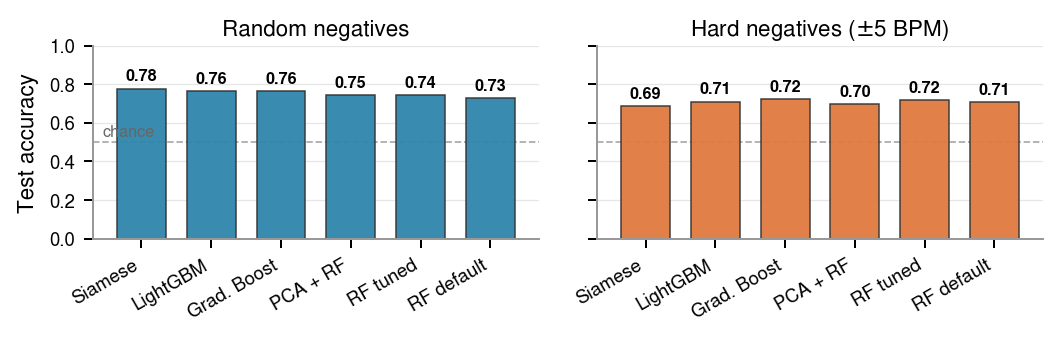
\includegraphics[width=\linewidth]{figures/model_accuracy.png}
    \subcaption{}
    \vspace{0.5em}
    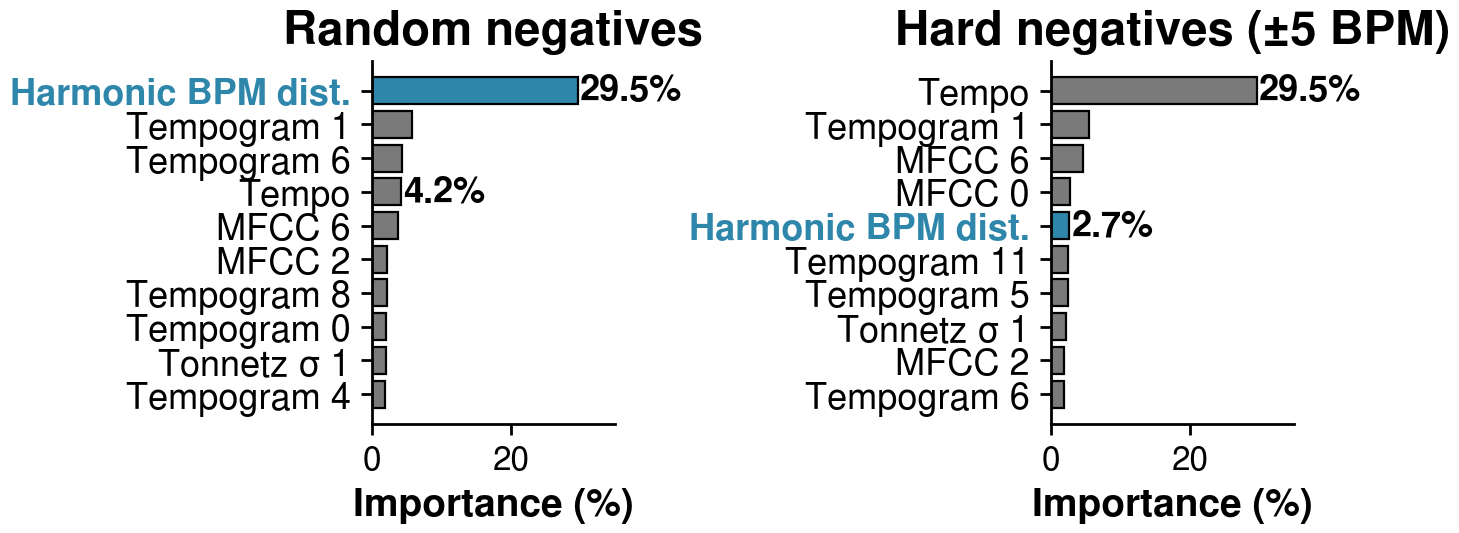
\includegraphics[width=\linewidth]{figures/feature_importance_gbm.png}
    \subcaption{}
  \end{minipage}%
  \hfill
  \begin{minipage}[c]{0.3\linewidth}
    \caption{\textbf{(a)} test accuracy across the six models under both negative-sampling regimes, sorted left to right by random-negative accuracy. Siamese is best on random and worst on hard; the dashed line is chance ($0.5$) on the balanced binary task. \textbf{(b)} Gradient Boosting feature importance, top 10 base features per regime (per-feature contributions from the $A$, $B$, and $|A - B|$ panels are summed). Under random negatives the harmonic BPM distance dominates at $29.5\%$. Under hard negatives ($\pm 5$ BPM) it collapses to $2.7\%$ (rank 5) and Tempo takes the top spot.}
    \label{fig:model-eval}
  \end{minipage}
\end{figure}




Retrieval metrics. On the same 668-query test corpus the Gradient Boosting recommender achieves a mean reciprocal rank of $0.042$, $\mathrm{recall}@5 = 0.043$, and $\mathrm{recall}@10 = 0.078$. The corresponding random-pick baselines are $\mathrm{recall}@5 = 0.0048$ and $\mathrm{recall}@10 = 0.0096$, so the model sits $8.9\times$ and $8.1\times$ above chance respectively. The median rank of the true next track is $114$ out of $1043$ candidates, and so on a typical query, the right answer is already inside the top $11\%$ of the ranking. Recall climbs to $0.276$ at $k = 50$, confirming that the model concentrates the truth toward the head of the list rather than dispersing it across the candidate pool.

\begin{figure}[H]
  \centering
  \begin{minipage}[c]{0.34\linewidth}
    \centering
    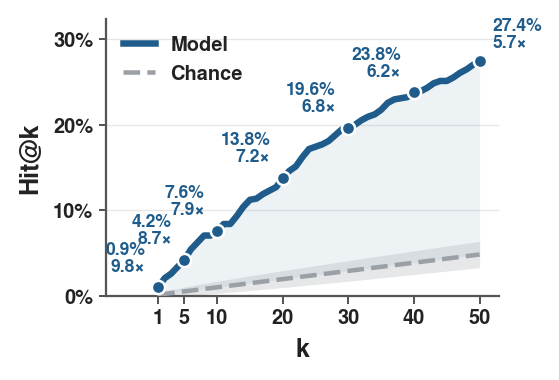
\includegraphics[width=\linewidth]{figures/hit_at_k_curve.png}
    \subcaption{}
  \end{minipage}%
  \hfill
  \begin{minipage}[c]{0.34\linewidth}
    \centering
    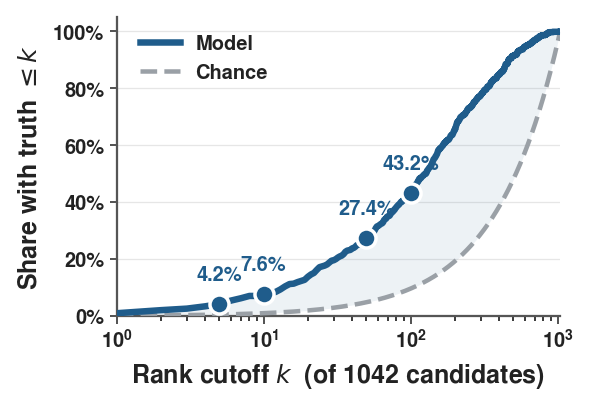
\includegraphics[width=\linewidth]{figures/rank_cdf.png}
    \subcaption{}
  \end{minipage}%
  \hfill
  \begin{minipage}[c]{0.30\linewidth}
    \centering
    \fbox{\parbox{\dimexpr\linewidth-2\fboxsep-2\fboxrule}{\footnotesize
      \textbf{Retrieval summary} \\[0.3ex]
      Mean reciprocal rank $= 0.042$\\($5.8\times$ chance) \\[0.3ex]
      Median rank $= 114 / 1042$ \\[0.3ex]
      $n = 741$ pairs, $668$ queries
    }}
    \subcaption{}
  \end{minipage}

  \caption{\textbf{(a)} Hit@$k$ on the held-out test corpus across $n = 741$ (query, true-next-track) pairs when the gradient-boosting model ranks all $1042$ test-corpus candidates by posterior. Each marker shows the share of queries whose truth lands in the top $k$ alongside the lift over a uniform random ranker. \textbf{(b)} cumulative distribution of the truth's rank across queries; the gap to the random baseline (dashed) is widest in the top $\sim 200$ ranks, then converges in the long tail. \textbf{(c)} headline retrieval statistics on the same test corpus.}
  \label{fig:hit-at-k}
\end{figure}

Moreover, in order to have a human evaluation, a survey was sent out consisting of five queries each one ranking the five most mixable songs. Users gave scores from $0$ to $5$, $0$ indicating no compatibility and $5$ indicating perfect mixability. The survey was completed by $35$ people, $20\%$ of whom are professional DJs, and some of whom are from the SoundCloud team. The five queries in the survey span distinct genres (see \Cref{ScoreHV}) so we could evaluate the model across multiple styles.


\begin{figure}[H]
  \centering
  \begin{minipage}[c]{0.62\linewidth}
    \centering
    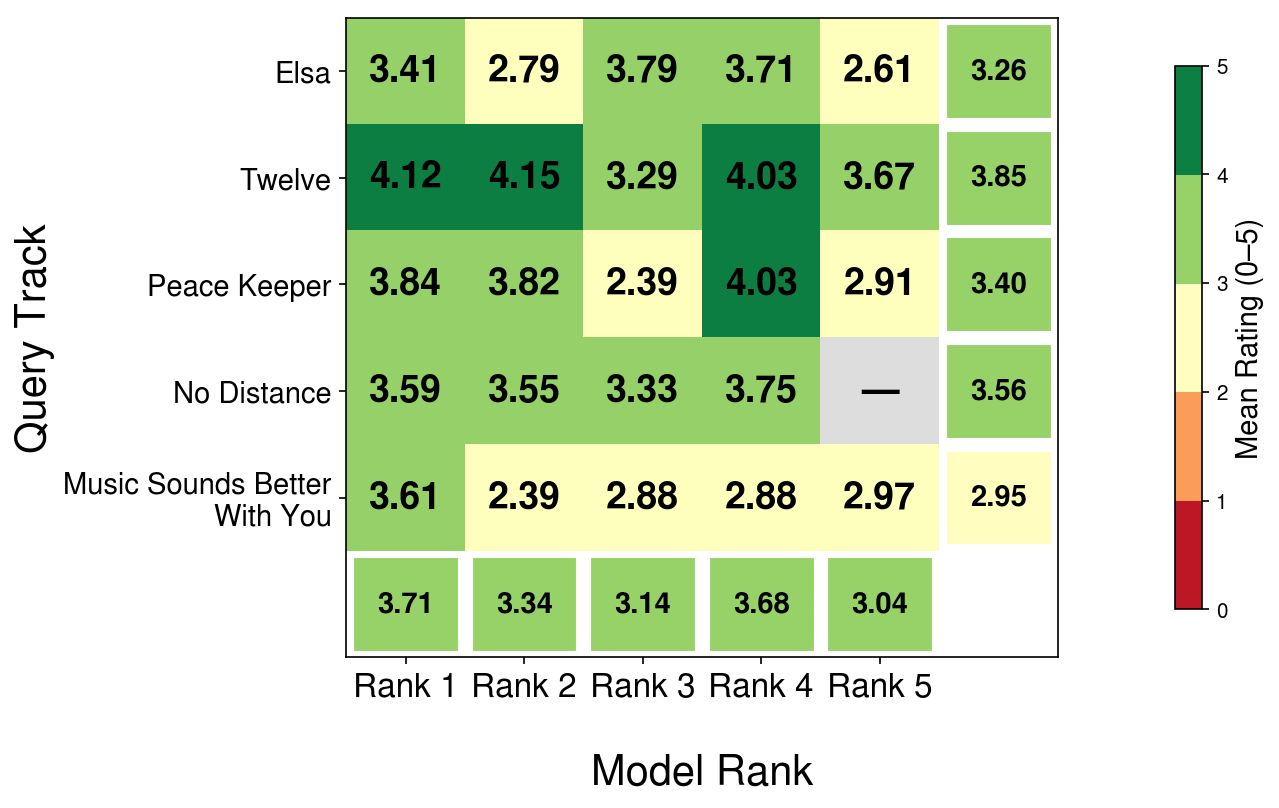
\includegraphics[width=\linewidth]{figures/query_rank_rating.png}
  \end{minipage}%
  \hfill
  \begin{minipage}[c]{0.36\linewidth}
    \caption{Per-query, per-rank mean survey rating on the original 0--5 scale averaged across raters. Each row is one of the five survey query tracks (genre in italics); the rightmost column is each track's mean across ranks and the bottom row is each rank's mean across tracks. Overall mean across all cells is $3.40$ ($67.84\%$ satisfaction). The Rank-5 cell for \textit{No Distance} was not collected.}
    \label{ScoreHV}
  \end{minipage}
\end{figure}
\vspace{-0.5em}

Results from the survey show an overall satisfaction of the model of $67.84\%$. As shown in \Cref{ScoreHV}, the song which received the highest score is \textit{Twelve - Psyk Rework} (Tech House), coherent with the fact that the training dataset is mainly Tech House dominated. The song with the lowest score is \textit{Music Sounds Better With You - Stardust} (Funky House), a genre absent from our training data, so the prediction is less accurate. The remaining three songs have similar scores between $3.26$ and $3.56$ on the 0--5 scale; their genres represent between $6.9\%$ and $18.7\%$ of the dataset. The score of a song increases with the share of its genre in the dataset, which is expected: the more similar songs the model has seen, the better its recommendations.

\section{Discussion \& Limitations}


\paragraph*{Negative sampling and redundant inductive bias.} The process of generating hard samples was trickier than expected. We tried sampling tracks that were close in BPM but harmonically incompatible, on the intuition that these would be the obvious wrong answers a DJ would never reach for. The problem is that BPM and harmonic compatibility were already part of the input feature vector, so the negatives were easily separable by the same signals the model was using on the positive side. From the results above the training accuracy of test results became worse, and instead random non-adjacent sampling yielded a better training signal, despite being less informative on paper. In the future, exploring a selective negative mining that targets dimensions such as timbre, mood, or rhythmic structure, which the current feature set captures less directly might be worthwhile to explore.

\paragraph*{Absence of a human baseline.} We have no human ground truth for what counts as mixable and no measurement of how a professional DJ performs on the same selection task. Without a head to head comparison, we cannot say whether the model is competitive with the humans it is meant to assist, which matters for product viability. Lavinia, who's a DJ, gave informal feedback as a sanity check, but a proper study would require recruiting working DJs or building a deployable evaluation tool. On the pairs Lavinia was able to extract, the CI was too large for a meaningful comparison to our models.

\paragraph*{Training on entire songs rather than mix sections.} 
We extract features from full tracks, but normally DJs mix on intros and outros. An improved pipeline would isolate the first and last 30 to 60 seconds of each track and learn compatibility from those segments, specifically. 

\paragraph*{Assumed bidirectionality of compatibility.} We treat $(A, B)$ and $(B, A)$ as equivalent, but mixing is directional. A track with a clean outro fits the outgoing role and one with a strong intro fits the incoming role, and the same pair often works in only one order. 

\paragraph*{Reliance on predefined genre imbalance.} Our dataset is heavily skewed toward Tech House, explaining why tracks from other genres such as Funky House consistently received worse compatibility scores than Tech House tracks, which is a direct symptom of the imbalance rather than a real signal about mixability. A larger and more genre balanced dataset would reduce this bias.

\paragraph*{Storage and memory constraints.} We downloaded around 30 GB of .mp3s, capping the size and diversity of our audio corpus. A larger corpus would not change the architecture but would likely improve generalization.



The full feature extraction code and pipeline is available at \url{https://github.com/jrafailov/musikal}.

\textit{The audio data were used solely for non-commercial academic experimentation and were not redistributed or made available outside the research setting. This use was intended to evaluate the feasibility DJ-transition modeling. All rights in the underlying recordings remain with their respective rightsholders.}

% compact bibliography spacing so References fit at the bottom of the
% Discussion page rather than getting pushed to a sparse page on their own
\setlength{\bibsep}{1pt plus 0.3ex}
\bibliographystyle{abbrvnat}
\setcitestyle{numbers}
\bibliography{references}





%%%%%%%%%%%%%%%%%%%%%%%%%%%%%%%%%%%%%%%%%%%%%%%%%%%%%%%%%%%%




%%%%%%%%%%%%%%%%%%%%%%%%%%%%%%%%%%%%%%%%%%%%%%%%%%%%%%%%%%%%

\end{document}
